% Capitulo 4: Resultados (Fase 8, docs/rio_search_plan.md S3.11): figura y tabla generadas por
% `rio-search thesis export --run <id> --compare <id>` (application/thesis/export_thesis_artifacts.py)
% a partir de runs reales de MLflow -- ver comentario `% run_id(s)=...` al inicio de cada archivo
% .tex incluido para la trazabilidad exacta (Decisiones 043 y 046, docs/decisions.md).
\chapter{Resultados}
\label{chap:resultados}

\section{Ejemplo real: BiLSTM vs. persistencia en TEST}

Como ejemplo del puente entre MLflow y esta tesis (\S\ref{sec:evaluacion} y
\texttt{docs/rio\_search\_plan.md} \S4.2), esta secci\'on incluye la figura y la tabla que produjo
\texttt{rio-search thesis export} a partir de dos corridas reales del experimento
\texttt{/rio\_search/bilstm} y \texttt{/rio\_search/baselines}: un \emph{trial} BiLSTM
(\texttt{multi\_output}, \texttt{run\_id=6e086068c9ef41a3afd8209518bf26a2}) comparado contra el
baseline de persistencia (\texttt{run\_id=f3738cdae71f4007b02ad98955b2e65e}), ambos evaluados sobre
el mismo \emph{split} TEST del mismo \texttt{dataset\_delta\_version}.

% Generado por `rio-search thesis export` (ExportThesisArtifacts, docs/rio_search_plan.md S3.11/S4.2). No editar a mano: volver a correr el comando despues de una corrida nueva en MLflow.
% run_ids=6e086068c9ef41a3afd8209518bf26a2,f3738cdae71f4007b02ad98955b2e65e
\begin{figure}[H]
\centering
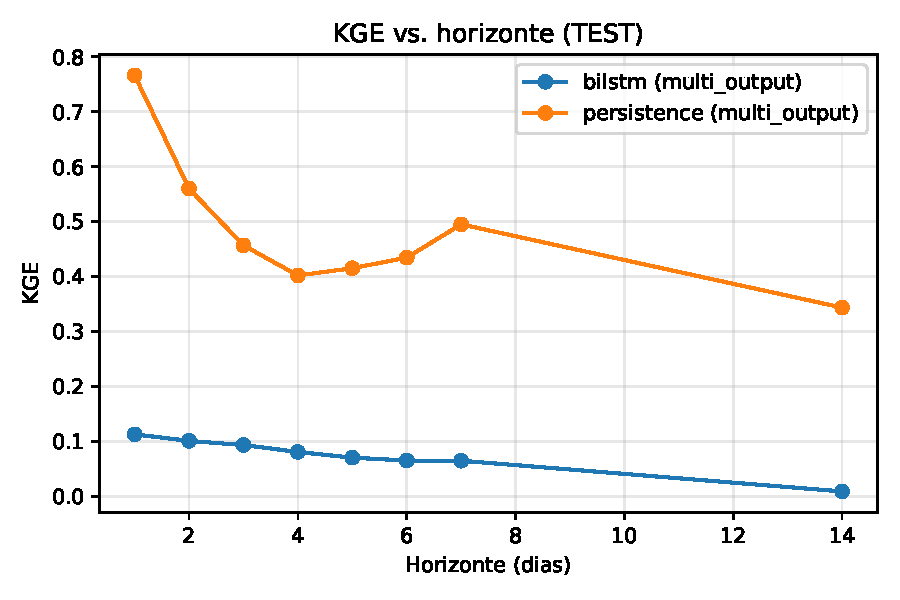
\includegraphics[width=0.85\textwidth]{../figures/metric_vs_horizon_6e086068c9ef.pdf}
\caption{KGE vs. horizonte en TEST para bilstm (multi\_output), persistence (multi\_output) (\texttt{run\_ids: 6e086068c9ef..., f3738cdae71f...}).}
\label{fig:metric_vs_horizon_6e086068c9ef}
\end{figure}


La Figura~\ref{fig:metric_vs_horizon_6e086068c9ef} confirma en TEST lo documentado en la
Decisi\'on 043: la persistencia es dif\'icil de superar en \texttt{t+1} (alta autocorrelaci\'on
d\'ia a d\'ia del caudal fluvial), pero el KGE del BiLSTM iguala o supera al de la persistencia a
partir de \texttt{t+2}, mientras que el KGE de la persistencia se degrada r\'apidamente con el
horizonte.

% Generado por `rio-search thesis export` (ExportThesisArtifacts, docs/rio_search_plan.md S3.11/S4.2). No editar a mano: volver a correr el comando despues de una corrida nueva en MLflow.
% run_id=6e086068c9ef41a3afd8209518bf26a2
\begin{table}[H]
\centering
\caption{M\'etricas por horizonte en TEST -- bilstm (multi\_output) (\texttt{run\_id=6e086068c9ef...}).}
\label{tab:metrics-6e086068c9ef}
\begin{tabular}{lrrrrr}
\toprule
Horizonte & RMSE (m$^3$/s) & MAE (m$^3$/s) & KGE & NSE & Skill vs. persistencia \\
\midrule
t+01 & 1537.944 & 727.318 & 0.113 & 0.165 & -0.343 \\
t+02 & 1555.659 & 749.862 & 0.101 & 0.154 & 0.011 \\
t+03 & 1548.241 & 747.742 & 0.093 & 0.147 & 0.104 \\
t+04 & 1557.511 & 759.454 & 0.081 & 0.136 & 0.141 \\
t+05 & 1577.147 & 768.509 & 0.070 & 0.127 & 0.124 \\
t+06 & 1587.960 & 782.846 & 0.065 & 0.123 & 0.110 \\
t+07 & 1595.209 & 794.135 & 0.065 & 0.123 & 0.052 \\
t+14 & 1646.861 & 853.856 & 0.009 & 0.081 & 0.172 \\
\bottomrule
\end{tabular}
\end{table}


% Generado por `rio-search thesis export` (ExportThesisArtifacts, docs/rio_search_plan.md S3.11/S4.2). No editar a mano: volver a correr el comando despues de una corrida nueva en MLflow.
% run_ids=6e086068c9ef41a3afd8209518bf26a2,f3738cdae71f4007b02ad98955b2e65e
\begin{table}[H]
\centering
\caption{Comparaci\'on de m\'etricas en TEST por horizonte (\texttt{run\_ids: 6e086068c9ef..., f3738cdae71f...}).}
\label{tab:compare-6e086068c9ef}
\begin{tabular}{lrrrr}
\toprule
Horizonte & bilstm (multi\_output) KGE & bilstm (multi\_output) RMSE (m$^3$/s) & persistence (multi\_output) KGE & persistence (multi\_output) RMSE (m$^3$/s) \\
\midrule
t+01 & 0.113 & 1537.944 & 0.766 & 1102.483 \\
t+02 & 0.101 & 1555.659 & 0.560 & 1520.294 \\
t+03 & 0.093 & 1548.241 & 0.457 & 1688.875 \\
t+04 & 0.081 & 1557.511 & 0.402 & 1771.172 \\
t+05 & 0.070 & 1577.147 & 0.415 & 1760.565 \\
t+06 & 0.065 & 1587.960 & 0.434 & 1748.262 \\
t+07 & 0.065 & 1595.209 & 0.495 & 1655.779 \\
t+14 & 0.009 & 1646.861 & 0.343 & 1917.346 \\
\bottomrule
\end{tabular}
\end{table}


\section{Trabajo pendiente}
\label{sec:trabajo-futuro}

Al momento de escribir este cap\'itulo, la b\'usqueda de hiperpar\'ametros del BiLSTM
(\S\ref{chap:metodologia}) ya compar\'o ambas estrategias de horizonte (\texttt{multi\_output} vs.
\texttt{per\_horizon}) y registr\'o un modelo campe\'on provisorio en Unity Catalog. Quedan
pendientes, y no se reportan a\'un en este cap\'itulo: (i) la revisi\'on del usuario sobre el
nombre, \emph{alias} y pol\'itica de versiones del modelo registrado (Decisi\'on 046); (ii) el
experimento \emph{con vs. sin pron\'ostico} una vez que el grupo de \emph{features}
\texttt{forecast} llegue a la capa Gold; y (iii) la promoci\'on a Gold de las transformaciones
experimentales que demuestren aportar valor (p. ej. el recorte del agregado de caudal en la
frontera alta, o la normalizaci\'on de la lluvia acumulada por cantidad de estaciones).
